\section{Results}
\label{sec:results}

\Cref{tbl:properties} shows the data used for these calculations. This data was extracted from various sources, as indicated in the table, and represents only preliminary estimates.

\begin{table}
    \centering
    \begin{tabular}{ccc}
    \toprule
    Property & Value & Source \\ \midrule
        $k_b$ &  1.5W/(m K) & \cite{thermalprop} \\
        $k_s$, aluminum & 238W/(m K) & \cite{thermalprop}\\
        $k_s$, CF, high conductivity & 60W/(m K) &\cite{silva2007plane} \\
        $k_s$, CF, low conductivity & 15W/(m K) &\cite{silva2007plane} \\
        $k$, air & $2.624\cdot10^{-5}\text{kW/(m K)}$ & \cite{kreith} \\
        $t_s$ & 1mm &\cite{roskam} \\
        $R_i$ & 0.5m$\Omega$ & \cite{thermalprop} \\
        $V_\text{cell}$& 2.1V & Oxys Energy\footnotemark \\
        $m_\text{cell}$& 0.137kg & Oxys Energy\\
        $\rho_b$ & 732 \si{kg/m^3} & Oxys Energy\\
        maximum operating temperature, pouch & 30\si{\celsius} & Oxys Energy\\
        $m_b$ & 150kg & CEA \\
        $P$ & 200\si{kW} & CEA \\
        $c$ & 0.814m & CEA \\
        $V_\infty$ (flight speed), typical & 90\si{m/s} & CEA \\
        Pr, air& 0.707 & \cite{kreith} \\
        $\mu$, air & $1.568\cdot10^{-5} \si{m^2/s}$ & \cite{kreith}\\
        $\rho$, air & 1.284 &\cite{kreith} \\
    \bottomrule
        
    \end{tabular}
    \caption{Inputs used to calculate results}
    \label{tbl:properties}
\end{table}
\subsection{The battery}
Following the procedure in \cref{sec:battery} and inputs from \cref{tbl:properties}:
\begin{align}
    N_\text{pouches} &= 1095 \\ 
    \dot{Q} &= 66.27\si{kW} \notag
\end{align}

The heat generated per unit volume is then
\begin{equation}
    \dot{q} = 271.17\si{kW/m^3}
\end{equation}

\subsection{Conduction cooling}
\label{subsec:cc}

Surface temperature can be estimated from the heat transfer coefficient as shown in \cref{sec:cc}.

The dimensions considered for each battery pack were $130\times 482 \times 650 \text{mm}$ ($t_b\times\text{length} \times\text{width}$), as suggested by Oxys Energy\footnote{\url{http://oxisenergy.com/wp-content/uploads/2016/08/OXIS-Rack-Mounted-Battery.pdf}}. 

Using the proposed relation for Nusselt, the convection coefficient and other relevant parameters are:
\begin{align}
\text{Re} &= 3\cdot10^6 \\
\text{Nu} &= 509\\
h         &= 32.83\si{W/m^2}
\end{align}

Differente ISA temperatures were considered at first for only one type of material --- Highly Conductive Carbon Fiber. The results can be seen in \cref{fig:surfacetemp}.
\begin{figure}
    \centering
    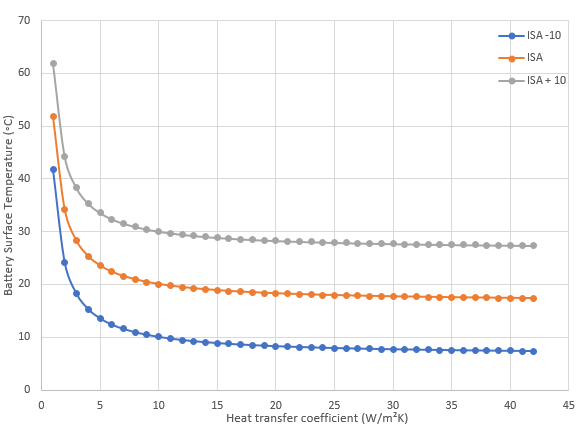
\includegraphics[width=\textwidth]{fig/carbon-isa.png}
    \caption{Surface temperature for different values of h atmospheric temperature - Material utilized was Highly Conductive Carbon Fiber.}
    \label{fig:surfacetemp}
\end{figure}

In order to evaluate the impact of different wing skin materials, the same conditions were applied for different materials --- same battery and skin thickness and also ISA+10. Results in \cref{fig:materials}.
\begin{figure}
    \centering
    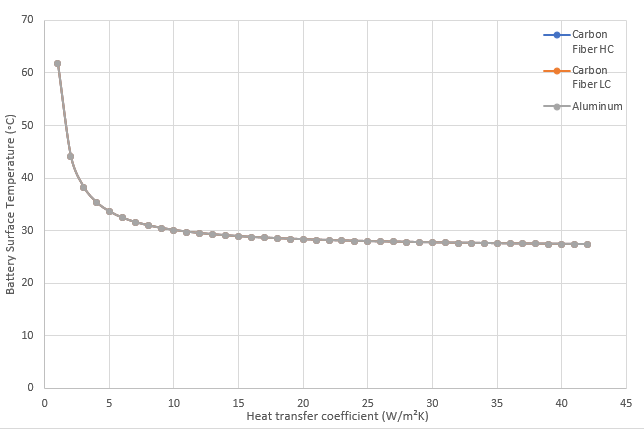
\includegraphics[width=\textwidth]{fig/materials.png}
    \caption{Surface temperature for different materials, ISA+10.}
    \label{fig:materials}
\end{figure}

Then battery thickness was also evaluated. For this condition, the same battery Area was considered, which means the pouches weren't rearranged, just given more (or less) space between rows.
Also, Carbon Fiber with High Conductivity was the chosen material. Results are shown in \cref{fig:bathick}.
\begin{figure}
    \centering
    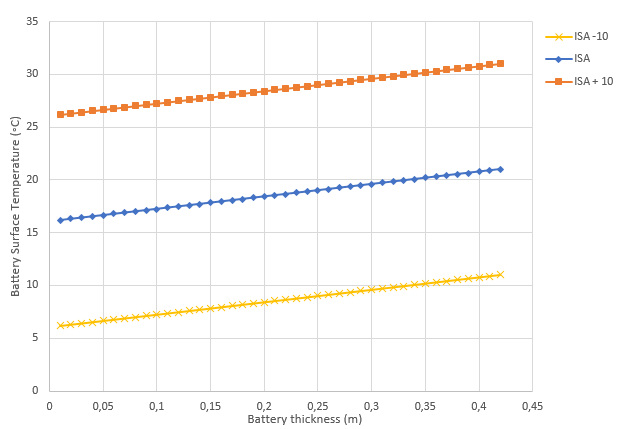
\includegraphics[width=\textwidth]{fig/bathick.png}
    \caption{Surface temperature for different values of battery thickness, ISA+10.}
    \label{fig:bathick}
\end{figure}


\subsection{Air cooling}

Following the procedure delineated in \cref{sec:air}, and \cref{subsec:cc} pack dimensions, the total surface area  and number of packs are
\begin{align}
    A &= 3.153\si{m^2} \\
    N &= 5 \\
\end{align}

Assuming $T_0=30\si{\celsius}$, $T_a = 25\si{\celsius}$ (ISA+10), and $t_a=t_b$, the required Nusselt number and consequent Reynolds number, mass flow and drag are
\begin{align}
    \text{Nu} &= 286 \\
    \text{Re} &= 40\cdot10^6 \\
    \dot{m} &= 1503\si{kg/s} \\
    D &= 71\si{kN}
\end{align}
